\documentclass[sigconf,nonacm]{acmart}
\setcopyright{none}
\settopmatter{printacmref=false}
\usepackage{seqsplit}
\newcommand{\hashtt}[1]{\texttt{\seqsplit{#1}}}
\makeatletter
\g@addto@macro{\UrlBreaks}{\do0\do1\do2\do3\do4\do5\do6\do7\do8\do9\do a\do b\do c\do d\do e\do f}
\makeatother
\emergencystretch=1.5em

\title{Empirical Validation of Benford's Law on Checksum-Verified World Bank Population Data}

\begin{document}
\begin{abstract}
Benford's Law predicts that leading significant digits in many naturally occurring numerical datasets follow \(P(D_1=d)=\log_{10}(1+1/d)\), rather than a uniform distribution. We evaluate this prediction as a compact reproducibility and data-audit artifact using an externally downloaded World Bank population dataset pinned to a specific Git commit and verified before analysis by SHA-256 checksum \hashtt{7d2dd6a17f5ed7916de1f89a9c116791e64d207f2e2f6ce47c57e1ab46f0088a}. The verified file contains 17,195 data rows, all of which were positive finite population values retained for analysis, with zero exclusions. The first significant digits show acceptable conformity under Nigrini's mean absolute deviation (MAD) criterion: first-digit MAD is 0.0073, with Pearson \(\chi^2=100.2\) on 8 degrees of freedom. The second significant digits also track the generalized Benford distribution, with MAD 0.0041 and \(\chi^2=49.3\) on 9 degrees of freedom. To test whether the procedure is discriminating rather than trivially accepting any input, we apply the same digit-extraction and scoring pipeline to deterministic synthetic controls of equal size. A one-order uniform negative control is classified as nonconforming (MAD 0.0603), while a log-uniform positive control is classified as close conformity (MAD 0.0016). Excluding aggregate World Bank series leaves the first-digit classification unchanged; when the panel is partitioned into four predeclared year blocks, three remain in the acceptable range and the earliest (1960--1979) is marginally acceptable. The resulting artifact demonstrates a fully auditable pattern for public-data Benford studies: immutable source reference, checksum-gated provenance, tested significant-digit extraction, deterministic controls, and reproducible tables and figures.
\end{abstract}

\maketitle

\section{Introduction}
\label{sec:intro}
Benford's Law is a striking regularity of many real numerical collections: the leading significant digit is often not uniformly distributed. Instead, for first digit \(d\in\{1,\ldots,9\}\), the predicted probability is
\begin{equation}
    P(D_1=d)=\log_{10}(1+1/d).
    \label{eq:benford1}
\end{equation}
Thus a leading digit of 1 is expected about 30.1\% of the time, while a leading digit of 9 is expected only about 4.6\% of the time. Because this distribution is closed-form and externally specified, Benford analysis is widely used as a lightweight screening tool in forensic accounting, election auditing, and data-quality review. Its evidentiary value is limited---conformity does not prove correctness, and nonconformity does not prove fraud---but it provides a useful, reproducible diagnostic for numerical datasets that plausibly span multiple orders of magnitude.

This paper treats Benford analysis as a reproducibility artifact rather than as a new statistical test. The motivating question is simple: given a real public dataset whose exact bytes are downloaded from an immutable source, can a deterministic pipeline verify the input, extract significant digits, reproduce the expected Benford regularities, and reject an intentionally non-Benford control? We study World Bank country/year population values distributed through the \texttt{datasets/population} community package. The input file is pinned to a specific Git commit, verified by SHA-256 checksum before any analysis, and accompanied by recorded provenance including source URL, retrieval timestamp, row count, byte count, schema, and attribution. This provenance-first design is central: because the evidence depends on an external dataset, the artifact is only meaningful if reviewers can confirm the exact input analyzed.

We evaluate three empirical questions. First, do the first significant digits of the population values conform practically to Benford's Law? Second, do the second significant digits follow the generalized Benford distribution? Third, does the same scoring procedure discriminate by rejecting a same-size synthetic control drawn uniformly over a single order of magnitude? By the practical effect-size criterion used here the answers are affirmative, although large-sample chi-square tests reject exact conformity at both digit positions (Section~\ref{sec:results}). The verified dataset contains 17,195 data rows; all are positive finite population values retained for analysis. The first-digit mean absolute deviation (MAD) from Benford expectation is 0.0073, which falls in Nigrini's ``acceptable conformity'' range, with Pearson \(\chi^2=100.2\) on 8 degrees of freedom. The second-digit MAD is smaller, 0.0041, with \(\chi^2=49.3\) on 9 degrees of freedom. In contrast, the fixed-seed one-order uniform negative control has first-digit MAD 0.0603 and is classified as nonconforming. A complementary log-uniform positive control is classified as close conformity.

The contribution is therefore a compact, auditable empirical note. It combines an immutable public-data reference, fail-closed checksum validation, unit-tested significant-digit extraction, standard Benford conformity statistics, deterministic positive and negative controls, robustness checks, and table-driven figures. The study is intentionally small and CPU-only, but it illustrates a broader pattern for reproducible data-audit artifacts: every reported number should be traceable to a verified input file, a tested transformation, and a deterministic output table.

\section{Background and Related Work}
\label{sec:background}
The first-digit phenomenon now called Benford's Law is usually traced to Newcomb's observation that logarithm-table pages for small leading digits were more worn than pages for large leading digits, and to Benford's later empirical compilation across heterogeneous numerical tables \cite{newcomb1881,benford1938}. In its modern first-digit form, the law states that the probability of first significant digit \(d\) is \(\log_{10}(1+1/d)\) for \(d\in\{1,\ldots,9\}\). The same logarithmic structure extends beyond the first digit. For the second significant digit \(d\in\{0,\ldots,9\}\), the generalized Benford probability is
\begin{equation}
    P(D_2=d)=\sum_{k=1}^{9}\log_{10}\left(1+\frac{1}{10k+d}\right).
    \label{eq:benford2}
\end{equation}
These probabilities provide fixed, non-fitted reference distributions, making Benford analysis attractive for reproducible audits: the expected values do not depend on estimating parameters from the dataset under study.

Benford conformity is most plausible for numerical measurements that span several orders of magnitude and arise from heterogeneous or multiplicative processes rather than from assigned identifiers, fixed-width codes, or deliberately bounded uniform draws. Hill's scale-mixture account explains why randomly selected distributions and scale-unbiased sampling can yield Benford-like significant digits, while subsequent surveys emphasize that there is no universal guarantee: conformity depends on the data-generating process, scale, spread, and mixing conditions \cite{hill1995,bergerhill2011}. Population panels are therefore a natural but nontrivial test case. Country and territory populations vary from small islands and territories to very large countries and global aggregates, and the longitudinal panel mixes many demographic scales. At the same time, observations are temporally correlated and may include regional or income-group aggregates, so conformity should be interpreted as a practical data-quality pattern rather than as evidence of independent draws from an ideal Benford multinomial model.

Two families of diagnostics are common in applied Benford work. Pearson's chi-square goodness-of-fit statistic compares observed digit counts with the Benford expected counts and is straightforward for the nine first-digit categories or ten second-digit categories. However, with large samples, even small practical deviations can yield very small \(p\)-values; the issue is amplified when observations are dependent, as in country-year population series. For that reason, forensic-accounting practice often supplements hypothesis tests with effect-size summaries. We use the mean absolute deviation (MAD) between observed and Benford proportions as the primary practical conformity measure. Following Nigrini-style first-digit thresholds, MAD below 0.006 is treated as close conformity, below 0.012 as acceptable conformity, below 0.015 as marginally acceptable conformity, and at or above 0.015 as nonconformity \cite{nigrini2012}. These ranges are practical screening heuristics, not universal critical values, but they are well matched to an artifact whose aim is auditable data-quality assessment rather than formal proof of a generative model.

The present study also draws on reproducible empirical-work norms for external data. Because the input is not generated inside the artifact, dataset provenance is part of the evidence. The World Bank population indicator is public open data, and the \texttt{datasets/population} community package provides a convenient tabular distribution of the values. We pin the raw file to a specific Git commit and verify its SHA-256 checksum, row count, and schema before analysis. This design separates two questions that are often conflated in small empirical studies: whether the bytes analyzed are exactly the intended public dataset, and whether the digit distributions computed from those bytes conform to the Benford reference laws.

\section{Dataset and Provenance}
\label{sec:dataset}
The empirical input is the total-population panel distributed by the \texttt{datasets/population} community package from World Bank Open Data. The artifact downloads a single CSV file from an immutable GitHub raw URL pinned to commit \hashtt{425fc447a53a26c767a15a7de60c4cc2478a0595}:
\begin{quote}\small
\url{https://raw.githubusercontent.com/datasets/population/425fc447a53a26c767a15a7de60c4cc2478a0595/data/population.csv}
\end{quote}
The file has four columns: \texttt{Country Name}, \texttt{Country Code}, \texttt{Year}, and \texttt{Value}. Each row records one country, territory, or aggregate World Bank series for one year, and \texttt{Value} is the population count used in the digit analysis. The verified file contains 17,195 data rows, or 17,196 lines including the header, and is 552,112 bytes. Its required SHA-256 digest is \hashtt{7d2dd6a17f5ed7916de1f89a9c116791e64d207f2e2f6ce47c57e1ab46f0088a}.

Provenance validation is a gate, not a descriptive afterthought. Before any digit extraction or statistical comparison is run, the pipeline downloads or reads the cached CSV, computes its SHA-256 digest over the raw bytes, checks the expected row count, and verifies the schema exactly. A mismatch in any of these fields causes the run to fail closed rather than producing analysis outputs. This behavior was validated both by the normal successful run and by an explicit wrong-checksum test, which exits with a nonzero status and prints a checksum-mismatch error before analysis. The design protects the central reproducibility claim: every reported statistic is conditional on the exact pinned input bytes, not merely on a dataset with a similar name.

The generated provenance record stores the source URL, UTC retrieval timestamp, checksum, byte count, row count, header schema, attribution, license/terms note, and software-version metadata. The retrieval timestamp is intentionally recorded in the run artifact rather than hard-coded in the paper text, because it changes when reviewers redownload the same immutable file. The dataset is attributed to World Bank Open Data via the \texttt{datasets/population} package; the artifact records the World Bank open-data attribution and license/terms note alongside the checksum so that source identity and reuse terms can be audited together.

\begin{table}[t]
\centering
\caption{Checksum-gated dataset provenance for the World Bank population CSV.}
\label{tab:dataset-provenance}
\begin{tabular}{@{}lp{0.68\columnwidth}@{}}
\toprule
Field & Verified value \\
\midrule
Source & Pinned \texttt{datasets/population} Git commit \\
Rows & 17,195 data rows \\
File lines & 17,196 including header \\
Bytes & 552,112 \\
Columns & Country Name, Country Code, Year, Value \\
SHA-256 & \hashtt{7d2dd6a17f5ed7916de1f89a9c116791e64d207f2e2f6ce47c57e1ab46f0088a} \\
Validation & Fail-closed checksum, schema, and row-count gate \\
\bottomrule
\end{tabular}
\end{table}

For the primary analysis we retain all rows in the verified CSV and analyze the \texttt{Value} column exactly as distributed. The main panel may include countries, territories, and aggregate World Bank series; rather than silently filtering these rows, the artifact reports the full-panel result first and treats aggregate exclusion as a sensitivity analysis. This choice preserves a simple provenance chain from the pinned file to the primary tables while still allowing the robustness section to assess whether aggregate World Bank entries drive the conclusion. In the verified file, all 17,195 \texttt{Value} entries are positive finite population values, so the primary dataset has 17,195 analyzed rows and zero exclusions.

\section{Methods}
\label{sec:methods}

\subsection{Significant-digit extraction}
Each value is parsed from its decimal text into an exact decimal number rather than a binary floating-point value, its sign is ignored, and the first and second significant digits are read from the normalized digit string. Integers, decimals below one, powers of ten, and scientific notation therefore share a single normalization path. Values that cannot carry a significant digit are excluded with an explicit reason code (zero, missing or blank, or non-finite), and exclusions are counted by reason so that analyzed plus excluded rows always equals the verified row count. For a valid value with only one significant digit, the second significant digit is recorded as 0. The extraction functions are unit-tested on representative integers, decimals, negative values, numeric strings, scientific notation, and every exclusion category; a second, independent standard-library implementation has its own suite of 5 unit tests, all of which pass. The same tested functions score the population data and every synthetic control.

\subsection{First- and second-digit conformity statistics}
For a sample of \(n\) analyzed values with \(c_d\) occurrences of digit \(d\), the observed proportion \(\hat p_d=c_d/n\) is compared with the Benford proportion \(p_d\) from Equation~\eqref{eq:benford1} (first digits, \(d\in\{1,\ldots,9\}\)) or Equation~\eqref{eq:benford2} (second digits, \(d\in\{0,\ldots,9\}\)). The two statistics are
\begin{equation}
  \mathrm{MAD}=\frac{1}{K}\sum_{d}\left|\hat p_d-p_d\right|,
  \qquad
  \chi^2=\sum_{d}\frac{(c_d-np_d)^2}{np_d},
\end{equation}
where \(K\) is the number of digit categories, and the chi-square statistic \cite{pearson1900} has \(K-1\) degrees of freedom (8 for first digits and 9 for second digits). The first-digit MAD is mapped to the Nigrini bands of Section~\ref{sec:background}: close conformity below 0.006, acceptable conformity below 0.012, marginally acceptable conformity below 0.015, and nonconformity at or above 0.015 \cite{nigrini2012}. These bands are defined for first digits, so the second-digit MAD is reported as an effect size without a band label.

The \(p\)-value is the upper-tail probability of the chi-square distribution, computed with the SciPy survival function when that library is installed. SciPy is optional: without it the \(p\)-value fields are recorded as null and every other output is unchanged. As an independent check, the second-digit \(p\)-value is also computed with a pure-Python regularized upper incomplete gamma function, together with the standardized residual \((c_d-np_d)/\sqrt{np_d}\) of each digit. We treat MAD as the primary conformity measure and the chi-square test as a secondary diagnostic, for the large-sample and dependence reasons given in Section~\ref{sec:background}.

\subsection{Controls}
To check that the scoring procedure can reject data, a negative control draws 17,195 integers (the analyzed sample size of the population data) uniformly from a single order of magnitude with fixed seed 20260717. One driver draws from \([1000,10000)\) and the main analysis script from \([10000,100000)\); both yield the same first-digit counts. Two further fixed-seed variants, implemented independently, draw uniform floating-point values on \([1000,9999]\) and on \([1,10)\). A one-order uniform draw is far from Benford-like, so a working procedure should classify it as nonconformity; the predeclared criterion is a first-digit MAD of at least 0.015. To check that the procedure can also accept data, a positive control draws 17,195 values \(X=10^U\) with \(U\) uniform on \([0,6]\), spanning 6 orders of magnitude, with fixed seed 424242. Such log-uniform data are Benford-distributed by construction, so a working procedure should report close conformity up to finite-sample noise. All controls pass through the same scoring function as the population data.

\subsection{Sensitivity analyses}
The full panel contains 265 distinct codes, including World Bank aggregates (regions, income and lending groups, demographic-dividend groups, and the world total) that are sums of other rows. Two country-only panels remove these aggregates and recompute both first- and second-digit statistics. The first uses a documented static list of 48 aggregate codes, removing 3,120 rows and leaving 14,075 rows from 217 codes. The second derives the aggregate list from World Bank country metadata (rows whose region is ``Aggregates''), which yields 47 codes; it differs from the static list only by keeping the code for fragile and conflict-affected situations. This panel removes 3,055 rows and leaves 14,140 rows from 218 codes. The derived code list is fixed by a SHA-256 digest. Finally, the first-digit analysis is repeated within four year blocks declared before scoring: 1960--1979, 1980--1999, 2000--2019, and 2020--2024. Because country-year values are temporally correlated, the block results are descriptive diagnostics rather than independent hypothesis tests.

\subsection{Reproducibility checks}
A single driver runs six steps in order: the digit-extraction, provenance-gate, and \(p\)-value unit tests; download and verification of the pinned file; the primary analysis; and figure generation. An offline smoke test then reruns the analysis twice from the cached, verified file without network access and compares SHA-256 hashes of the 3 numeric outputs (the two digit tables and the summary record). Figures are drawn only from the saved result tables; a figure manifest records the byte count and SHA-256 digest of each figure and of its source table, and a smoke script fails if a table is missing or malformed, the manifest or a figure is missing or empty, or a byte count or digest does not match. A provenance appendix table is rendered deterministically from the recorded provenance and summary files.

\section{Results}
\label{sec:results}

\begin{table*}[t]
\centering
\caption{Conformity statistics for the population data and the synthetic controls. MAD values are rounded to six decimal places and \(\chi^2\) to one; ``n/r'' means not recorded. All samples contain 17,195 values with zero exclusions.}
\label{tab:primary}
\begin{tabular}{llrrrl}
\toprule
Sample & Digit & MAD & \(\chi^2\) & dof & First-digit class / \(p\)-value \\
\midrule
Population & first & 0.007315 & 100.2 & 8 & acceptable conformity; \(p=3.9\times10^{-18}\) \\
Population & second & 0.004058 & 49.3 & 9 & no band; \(p=1.5\times10^{-7}\) \\
Negative control, integers on \([1000,10000)\) & first & 0.060256 & 6978.6 & 8 & nonconformity; \(p\) underflows to 0 \\
Negative control, floats on \([1000,9999]\) & first & 0.060889 & 6897.7 & 8 & nonconformity; n/r \\
Negative control, floats on \([1,10)\) & first & 0.060501 & 7312.3 & 8 & nonconformity; n/r \\
Positive control, log-uniform & first & 0.001621 & 6.2 & 8 & close conformity; n/r \\
\bottomrule
\end{tabular}
\end{table*}

\subsection{Population data}
Table~\ref{tab:primary} summarizes the main statistics. All 17,195 rows were analyzed, none were excluded, and no value needed the one-significant-digit convention. The first-digit MAD of 0.0073 lies in the acceptable-conformity band. Figure~\ref{fig:first} shows where the departures occur: leading 1s are under-represented (28.3\% observed against 30.1\% expected), while leading 5s (9.3\% against 7.9\%) and 4s (10.7\% against 9.7\%) are over-represented; every other digit deviates from its Benford proportion by at most 0.73 percentage points (digit 2). The chi-square statistic, 100.2 on 8 degrees of freedom (\(p=3.9\times10^{-18}\)), rejects exact Benford conformity.

\begin{figure}[t]
\centering
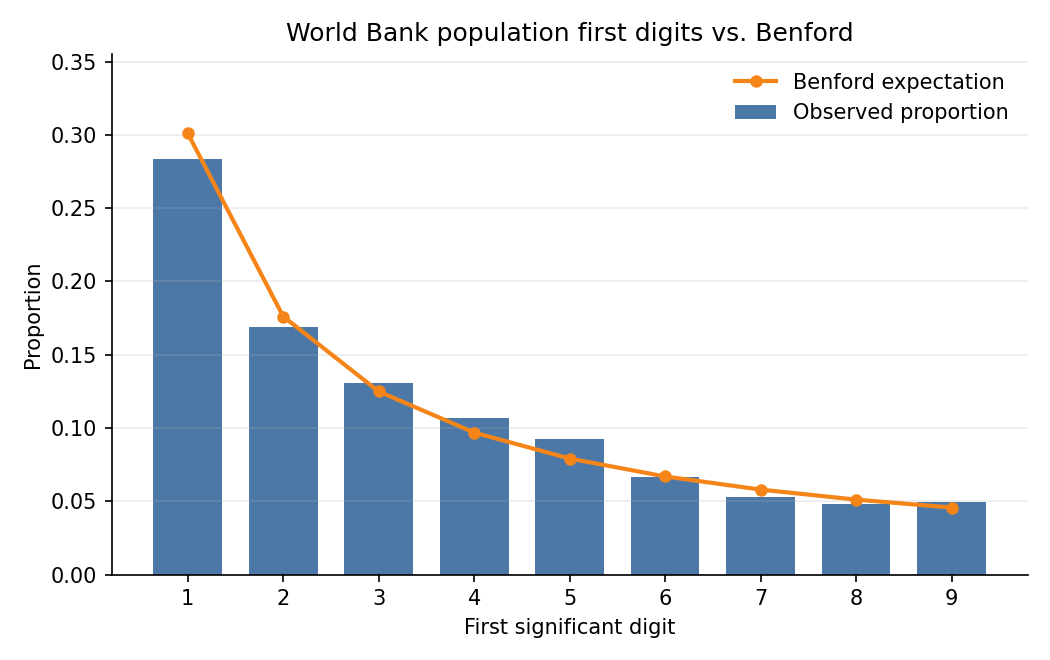
\includegraphics[width=\columnwidth]{reference-outputs/figures/first_digit_benford.png}
\caption{Observed first-digit proportions of the 17,195 population values (bars) against the Benford proportions (line).}
\label{fig:first}
\Description{Bar chart of observed first-digit proportions for digits 1 to 9 with the Benford curve overlaid.}
\end{figure}

The second-digit MAD is smaller, 0.0041, although the two MADs are not directly comparable because the second-digit distribution is much flatter than the first-digit one. The chi-square statistic is 49.3 on 9 degrees of freedom (\(p=1.5\times10^{-7}\)), again rejecting exact conformity. The standardized residuals (Figure~\ref{fig:second}) show that the rejection is concentrated in one digit: a second digit of 0 occurs 13.4\% of the time against 12.0\% expected (residual \(+5.56\)), and the next largest residuals are for digits 5 (\(-2.83\)) and 4 (\(-2.16\)); the remaining seven residuals lie between \(-1.53\) and \(0.74\). The independent pure-Python \(p\)-value agrees with the library value (\(1.5\times10^{-7}\) in both cases).

\begin{figure}[t]
\centering
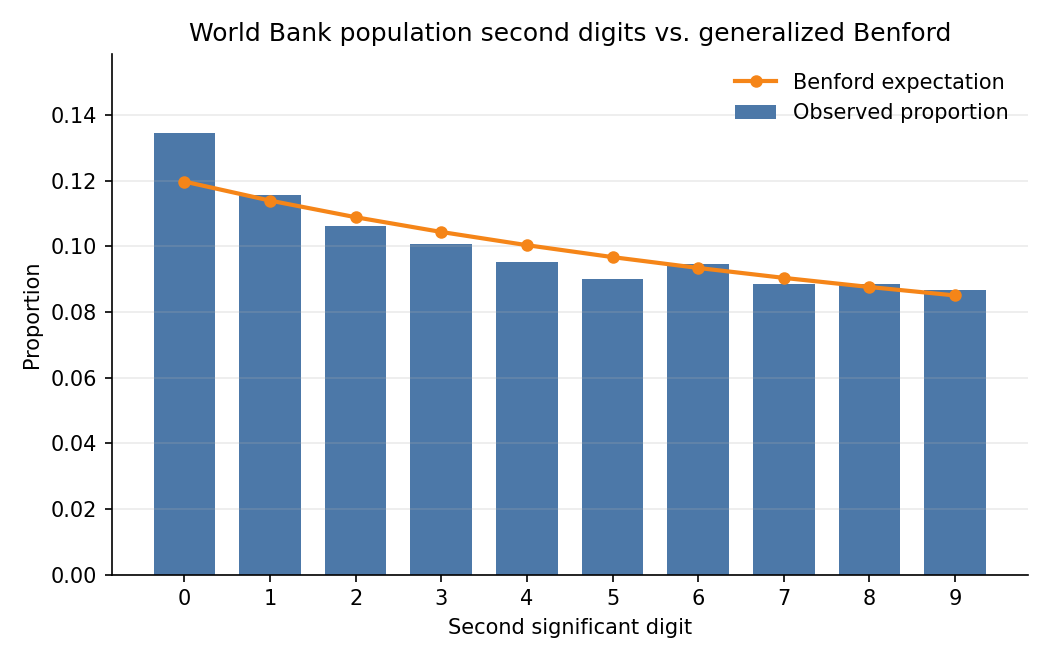
\includegraphics[width=\columnwidth]{reference-outputs/figures/second_digit_benford.png}
\caption{Observed second-digit proportions of the population values (bars) against the generalized Benford proportions (line).}
\label{fig:second}
\Description{Bar chart of observed second-digit proportions for digits 0 to 9 with the generalized Benford curve overlaid.}
\end{figure}

The two statistics therefore answer different questions. With 17,195 values, many of them repeated measurements of the same country in adjacent years, the chi-square test detects per-digit departures as small as those visible in Figures~\ref{fig:first} and~\ref{fig:second}, which the MAD criterion regards as practically small. The population data are Benford-like in the practical sense used in forensic screening, but they are not an exact draw from the Benford distribution.

\subsection{Controls}
The procedure discriminates in both directions (Table~\ref{tab:primary}). The integer negative control has first-digit MAD 0.0603, well inside the nonconformity band; its leading digit is 1 in only 11.1\% of draws against 30.1\% under Benford, and its \(p\)-value underflows to zero. The two floating-point variants agree: MAD 0.0609 and 0.0605, both nonconformity. A separate minimal rerun of the integer control reproduced the same MAD and classification. The log-uniform positive control is classified as close conformity, with MAD 0.0016 and \(\chi^2=6.2\) on 8 degrees of freedom; its leading digit is 1 in 29.7\% of draws. The real data thus sit between a sample that is Benford by construction and one that is clearly not, and the same code scores all three.

\subsection{Sensitivity analyses}

\begin{table}[t]
\centering
\caption{Sensitivity of the conformity results. MAD values are rounded to six decimal places; the class applies to the first-digit MAD.}
\label{tab:sensitivity}
\small
\setlength{\tabcolsep}{4pt}
\begin{tabular}{@{}lrrlr@{}}
\toprule
Panel & Rows & 1st MAD & Class & 2nd MAD \\
\midrule
Full panel & 17,195 & 0.007315 & acceptable & 0.004058 \\
Country-only (static) & 14,075 & 0.007368 & acceptable & 0.004879 \\
Country-only (metadata) & 14,140 & 0.007540 & acceptable & 0.004864 \\
\midrule
1960--1979 & 5,280 & 0.012916 & marginal & -- \\
1980--1999 & 5,290 & 0.010819 & acceptable & -- \\
2000--2019 & 5,300 & 0.008670 & acceptable & -- \\
2020--2024 & 1,325 & 0.010653 & acceptable & -- \\
\bottomrule
\end{tabular}
\end{table}

Removing aggregate series barely changes the result (Table~\ref{tab:sensitivity}). With the static list the first-digit MAD moves from 0.0073 to 0.0074 (\(\chi^2=95.3\)) and the second-digit MAD from 0.0041 to 0.0049 (\(\chi^2=50.4\)); with the metadata-derived list the values are 0.0075 (\(\chi^2=98.7\)) and 0.0049 (\(\chi^2=50.3\)). Every country-only first-digit result remains acceptable conformity, so the main conclusion is not driven by the aggregate rows.

The temporal picture is less uniform (Figure~\ref{fig:blocks}). Three of the four year blocks are in the acceptable band, but the earliest block, 1960--1979, has MAD 0.0129 and is only marginally acceptable. Every block also has a larger MAD than the pooled panel; smaller samples are one possible contributor, but the analysis does not separate sampling noise from genuine change over time. We read this as evidence that the pooled result does not depend on a single period, not as evidence of stable conformity in every period.

\begin{figure}[t]
\centering
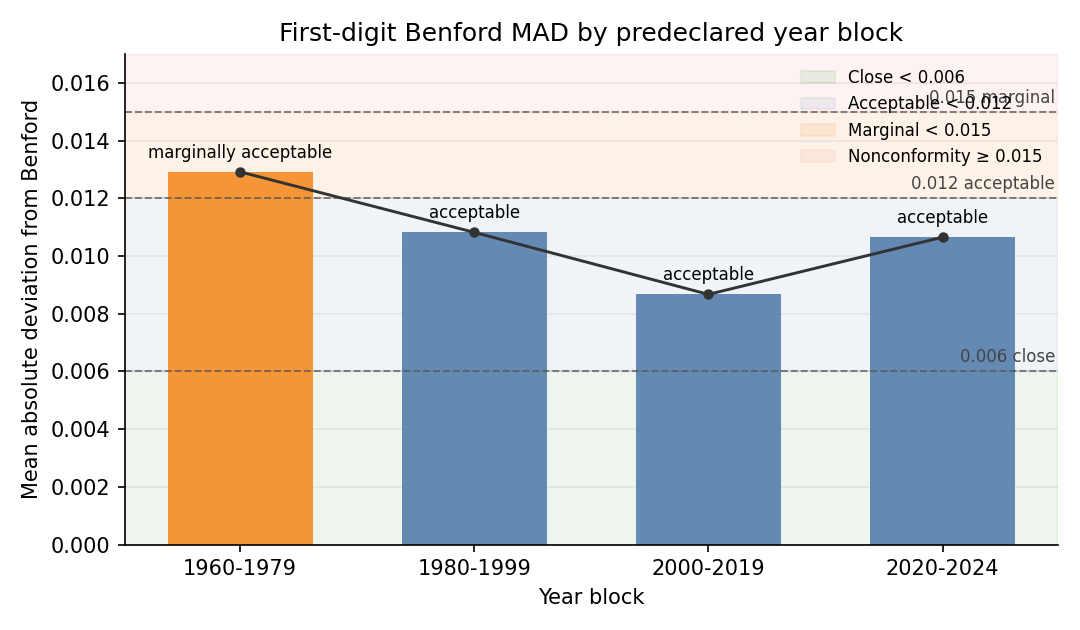
\includegraphics[width=\columnwidth]{reference-outputs/figures/year_block_mad.png}
\caption{First-digit MAD by predeclared year block, with the Nigrini bands shaded. The 1960--1979 block is marginally acceptable; the other three blocks are acceptable.}
\label{fig:blocks}
\Description{Bar chart of first-digit MAD for four year blocks with shaded Nigrini conformity bands.}
\end{figure}

\subsection{Reproducibility}
All six driver steps completed successfully, and the two offline reruns produced identical SHA-256 hashes for all 3 numeric outputs without network access. Both required figures were regenerated from the saved tables, the figure manifest matched, and the figure smoke test passed. The run without SciPy recorded null \(p\)-values and otherwise produced the same statistics. A clean container run with no host directories mounted downloaded and verified the pinned file, passed the unit tests, and reproduced the same key statistics. Both digit-extraction test suites passed, and invalid inputs were excluded with their reason codes.

\section{Threats to Validity and Limitations}
\label{sec:limitations}

\paragraph{Dependent observations.} The panel follows the same countries over time, so observations are neither independent nor identically distributed. The chi-square \(p\)-values are therefore not calibrated, and the very small values above should be read as signs of large-sample sensitivity, not as precise error rates. The MAD bands are practitioner heuristics, not critical values derived for this setting.

\paragraph{Aggregate rows.} Aggregates are sums of other rows and partly duplicate them. The country-only panels address this, but the static and metadata-derived code lists differ by one code. The metadata come from a live World Bank interface whose response has changed since the analysis, so the derived list is carried as a fixed, hash-verified list rather than being re-derived from the live interface.

\paragraph{Scope.} The study covers one dataset in one domain. Conformity of population counts says nothing about other indicators, and, as noted in Section~\ref{sec:intro}, Benford conformity is neither proof of data correctness nor evidence of manipulation when absent. The checksum guarantees the bytes of the pinned community redistribution, not that this redistribution matches the World Bank's current release, which may be revised over time.

\paragraph{Controls and labels.} The negative controls differ across scripts in range and number type; all are nonconforming, but their MADs differ slightly, and we report each one. The positive control shows that the procedure accepts ideal Benford data; it does not show how the procedure behaves on near-Benford data with realistic structure. One auxiliary validation script labels the second-digit MAD with the first-digit bands; we do not use that label. The one-significant-digit convention for second digits is unit-tested but never triggered by the population data.

\paragraph{Temporal and software variation.} One of four year blocks is only marginally acceptable, and the block analysis is descriptive. The SciPy version used for the \(p\)-values was not recorded, so \(p\)-values are reproducible to a small relative tolerance rather than bit-for-bit. The recorded environment used Python 3.10.12, NumPy 2.2.6, pandas 2.3.3, and Matplotlib 3.10.8.

\section{Conclusion}
World Bank country-year population counts are Benford-like in practice: the first digits fall in Nigrini's acceptable band and the second digits track the generalized Benford law with a small MAD, while the same procedure rejects a non-Benford control of equal size and accepts a Benford-by-construction control. Large-sample chi-square tests nevertheless reject exact conformity, and one early period is only marginally acceptable, so the result supports Benford analysis as a practical screen for this kind of data, not as a precise distributional model. For practitioners, the transferable lessons are to pin and checksum external inputs before analysis, to test digit extraction separately, to run positive and negative controls through the same scoring code, and to report an effect size such as MAD alongside any \(p\)-value.

\section*{Artifact Availability}
The accompanying artifact contains, for every analysis step, a specification detailed enough to re-implement the code and reproduce the reported numbers (the \texttt{specs/} directory, starting from its index), a data recipe (\texttt{DATA.md}) giving the pinned download address, SHA-256 digest, byte count, and row count of the input, the reference output tables and figures from which every number in this paper is taken, and a checksum list covering all shipped files. No data files are redistributed; network access is needed only for the pinned download, and all steps run on a CPU.

\bibliographystyle{ACM-Reference-Format}
\bibliography{references}

\end{document}
